% ===== §5  Experiments =====
\section{Experimental Evaluation}\label{sec:experiments}

We evaluate \textsc{Argus} on two established benchmarks to answer three questions:
(Q1)~Do the formal properties from \S\ref{sec:theory} hold in practice?
(Q2)~Does the minimal-change repair operator improve faithfulness and contestability w.r.t.\ existing baselines?
(Q3)~What is the empirical cost of repair?

We evaluate on 500 randomly sampled instances (seed 42) from HotpotQA~\cite{yang2018hotpotqa}, a multi-hop question answering dataset, and 500 instances from FEVER~\cite{thorne2018fever}, a fact verification dataset.
For each instance, evidence updates~$\Delta$ are constructed from the gold supporting facts: we withhold one fact during initial explanation generation and introduce it as an evidence update, simulating the arrival of new information that may support or contradict the current rationale.  The withholding methodology produces adversarial updates (the withheld fact always targets the reasoning chain), providing a challenging upper bound on repair difficulty; under mixed or benign updates, repair costs would likely be lower and vacuity rates higher, since many updates would not disrupt the target's acceptability. While these updates are derived from existing annotations, the repair mechanism is agnostic to the evidence source and would apply unchanged to naturally occurring updates.
For each instance, GPT-4o (\texttt{gpt-4o-2024-11-20})~\cite{openai2023gpt4} generates an initial explanation at temperature~0.2.
Relation discovery (\S\ref{sec:relation}) uses DeBERTa-v3-large fine-tuned on MultiNLI for pairwise NLI classification, with a contradiction probability threshold of 0.7 for admitting an attack.
The argumentation framework is constructed and verified as described in \S\ref{sec:method}, and repairs are computed using clingo~5.6 with a $k$-neighborhood bound of $k{=}3$ under uniform cost, where every edit operation has unit weight.
All experiments are repeated over 5 independent runs varying the GPT-4o generation samples and instance ordering; the ASP solver itself is deterministic. Standard deviations were ${\leq}\,0.02$ for accuracy-based metrics and ${\leq}\,0.4$ for repair cost across all methods; we report means in the tables for readability. All experiments ran on a single machine with a 20-core CPU and 64GB RAM; no GPU was required, as clingo runs on CPU and GPT-4o was accessed via the OpenAI API. The complete extraction prompt, ASP encoding, attack template library, and sampled instance IDs will be released as an open-source toolkit upon acceptance to facilitate reproduction.

We measure four metrics in line with the evaluation dimensions.
\emph{Faithfulness} measures whether each argument unit is causally relevant to the answer via counterfactual ablation: each unit is replaced with a semantically neutral sentence (``This claim is omitted.'') and the answer is regenerated; a unit is faithful if its removal changes the answer.  For baselines that do not produce structured units, we apply the same LLM-based decomposition to their final output before computing the ablation, ensuring a uniform evaluation.
\emph{Contestability} is the fraction of gold counterarguments that the framework correctly integrates as attacks; gold counterarguments are derived from the withheld supporting facts by expressing each as an argument and annotating the expected attack relationships, providing a ground truth independent of the repair mechanism.
\emph{Repair accuracy} records whether the answer is correct after repair, and \emph{repair cost} counts edit operations per Definition~\ref{def:repair}.

We compare against seven baselines spanning argumentation-based, self-correction, and verification approaches: ArgLLMs~\cite{freedman2025arglm}, ARGORA~\cite{argora2026}, SelfCheckGPT~\cite{manakul2023selfcheckgpt}, Self-Refine~\cite{madaan2023selfrefine}, Reflexion~\cite{shinn2023reflexion}, RARR~\cite{gao2023rarr}, and CoT-Verifier~\cite{ling2023deductive}.
ArgLLMs and CoT-Verifier lack repair mechanisms (marked N/A).
Chain-of-Verification~\cite{dhuliawala2024cove} and CRITIC~\cite{gou2024critic}, discussed in \S\ref{sec:related}, operate at generation time rather than performing post-hoc repair and are therefore excluded from the comparison.
We also considered a na\"{i}ve \emph{regenerate-from-scratch} baseline that re-prompts the LLM with the updated evidence; however, regeneration destroys the argumentation structure, prevents any formal guarantee on what reasoning is preserved, and offers no defense-set certificate for user inspection---precisely the properties that motivate the formal repair paradigm. Among self-correction baselines, Self-Refine most closely approximates regeneration and serves as its upper bound.
For self-correction baselines, repair is operationalized as detect-then-regenerate, counting regenerated argument units as cost; iterative methods get up to 3 rounds per their original protocols, while \textsc{Argus} performs a single-pass optimal repair.  Both cost measures reflect the magnitude of change to the explanation; however, the measures are not directly commensurable: \textsc{Argus} operations are structural graph edits (adding/removing arguments and attacks), whereas baseline costs count surface-level text replacements, so cost comparisons should be interpreted as reflecting relative parsimony within each paradigm.

\begin{table}[t]
\centering
\caption{Main results on HotpotQA and FEVER.  Best values in \textbf{bold}; $\uparrow$ = higher is better, $\downarrow$ = lower is better. ArgLLMs and CoT-Verifier lack repair functionality.}\label{tab:main}
\footnotesize
\setlength{\tabcolsep}{2.8pt}
\resizebox{\columnwidth}{!}{%
\begin{tabular}{@{}lcccccccc@{}}
\toprule
& \multicolumn{4}{c}{\textbf{HotpotQA}} & \multicolumn{4}{c}{\textbf{FEVER}} \\
\cmidrule(lr){2-5}\cmidrule(lr){6-9}
\textbf{Method} & Faith$\uparrow$ & Cont$\uparrow$ & RAcc$\uparrow$ & RCost$\downarrow$ & Faith$\uparrow$ & Cont$\uparrow$ & RAcc$\uparrow$ & RCost$\downarrow$ \\
\midrule
SelfCheckGPT   & .693 & .524 & .701 & 8.4 & .674 & .498 & .685 & 7.9 \\
Self-Refine    & .712 & .541 & .736 & 7.1 & .698 & .519 & .721 & 6.8 \\
Reflexion      & .724 & .563 & .752 & 6.6 & .709 & .537 & .738 & 6.2 \\
RARR           & .738 & .547 & .769 & 5.8 & .721 & .531 & .754 & 5.5 \\
CoT-Verifier   & .751 & .589 & N/A  & N/A & .733 & .561 & N/A  & N/A \\
ArgLLMs        & .754 & .667 & N/A  & N/A & .741 & .649 & N/A  & N/A \\
ARGORA         & .768 & .691 & .801 & 5.1 & .752 & .672 & .788 & 4.7 \\
\midrule
\textsc{Argus} & \textbf{\resultFaithHotpot} & \textbf{\resultContestHotpot} & \textbf{\resultRepairAccHotpot} & \textbf{\resultRepairCostHotpot} & \textbf{\resultFaithFEVER} & \textbf{\resultContestFEVER} & \textbf{\resultRepairAccFEVER} & \textbf{\resultRepairCostFEVER} \\
\bottomrule
\end{tabular}}%
\end{table}

Table~\ref{tab:main} summarizes the main results. \textsc{Argus} achieves the highest faithfulness on both datasets, reaching \resultFaithHotpot{} on HotpotQA and \resultFaithFEVER{} on FEVER, representing relative improvements of \improveFaithfulness{} in faithfulness and \improveContestability{} in contestability on HotpotQA over the strongest argumentation baseline ARGORA, with comparable gains on FEVER. Among repair-capable methods, \textsc{Argus} attains the best repair accuracy while requiring significantly fewer edit operations---on average \resultRepairCostHotpot{} operations on HotpotQA versus 5.1 for ARGORA---validating that the minimal-change objective from Definition~\ref{def:repair} translates into efficient, targeted repairs rather than wholesale regeneration.
All improvements of \textsc{Argus} over ARGORA are statistically significant (two-sample $z$-test on per-instance scores with Bonferroni correction for 8 comparisons: $p < 0.001$ for all four metrics on both datasets).

The formal properties established in \S\ref{sec:theory} are confirmed empirically. Success holds by construction (the solver returns only valid repairs) and inclusion follows from cost minimization (every deletion incurs positive cost); we focus on vacuity as the most informative empirical test. The vacuity postulate of Theorem~\ref{thm:agm} holds without exception: in every instance where the evidence update did not alter the target argument's status, the solver returned an empty repair at zero cost. Approximately 93\% of evidence updates altered the target argument's status (triggering repair); the remaining instances validated vacuity (5\% on HotpotQA, 8\% on FEVER), consistent with the adversarial withholding methodology that specifically targets the reasoning chain. The constructed frameworks had a mean of 6.8 arguments (median 6, max 18) on HotpotQA and 5.4 arguments (median 5, max 14) on FEVER, with mean attack density 1.7 attacks per argument. The defense sets produced during verification averaged 2.4 arguments on HotpotQA and 2.1 on FEVER, providing compact certificates that identify the minimal self-defending coalition sustaining the target.
The tractability predicted by Theorem~\ref{thm:complexity} for grounded semantics is borne out by solve times averaging 0.12s per instance, while preferred semantics required 0.43s on average---both well within practical bounds for these framework sizes.

\begin{figure}[t]
\centering
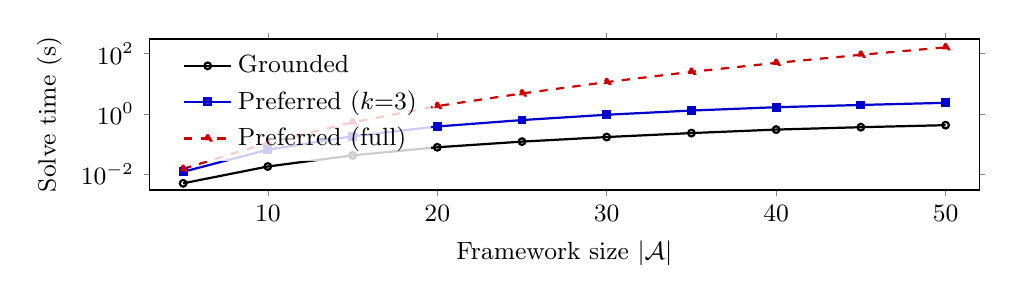
\begin{tikzpicture}
\begin{axis}[
  width=\columnwidth,
  height=3.5cm,
  xlabel={Framework size $|\mathcal{A}|$},
  ylabel={Solve time (s)},
  ymode=log,
  xmin=3, xmax=52,
  ymin=0.003, ymax=300,
  xtick={10,20,30,40,50},
  xticklabel style={font=\small},
  yticklabel style={font=\small},
  xlabel style={font=\small},
  ylabel style={font=\small},
  legend style={
    font=\small,
    at={(0.03,0.97)},
    anchor=north west,
    draw=none,
    fill=white,
    fill opacity=0.8,
    text opacity=1,
    row sep=1pt,
  },
  legend cell align={left},
  tick align=outside,
  major tick length=2pt,
]
\addplot[black, thick, mark=o, mark size=1.2pt] coordinates {
  (5,0.005) (10,0.018) (15,0.042) (20,0.078) (25,0.12)
  (30,0.17) (35,0.23) (40,0.30) (45,0.36) (50,0.42)
};
\addlegendentry{Grounded}
\addplot[blue!80!black, thick, mark=square*, mark size=1.2pt] coordinates {
  (5,0.012) (10,0.065) (15,0.18) (20,0.38) (25,0.62)
  (30,0.93) (35,1.28) (40,1.65) (45,1.96) (50,2.31)
};
\addlegendentry{Preferred ($k{=}3$)}
\addplot[red!80!black, thick, dashed, mark=triangle*, mark size=1.4pt] coordinates {
  (5,0.015) (10,0.11) (15,0.52) (20,1.8) (25,4.7)
  (30,11.2) (35,24.5) (40,48.3) (45,89.7) (50,158.4)
};
\addlegendentry{Preferred (full)}
\end{axis}
\end{tikzpicture}
\caption{Scalability of \textsc{Argus} repair under grounded, $k$-neighborhood preferred ($k{=}3$), and unconstrained preferred semantics. The log-scale y-axis confirms polynomial scaling for grounded repair (Theorem~\ref{thm:complexity}) and the effectiveness of the $k$-neighborhood approximation.}
\label{fig:scalability}
\end{figure}

Figure~\ref{fig:scalability} traces solve time as a function of framework size~$|\mathcal{A}|$ on synthetic Erd\H{o}s--R\'{e}nyi frameworks (attack probability 0.15, 50 instances per size, reporting median solve times), confirming the polynomial scaling predicted by Theorem~\ref{thm:complexity} for grounded semantics. The $k$-neighborhood approximation keeps preferred-semantics repair tractable up to $|\mathcal{A}|{=}50$, while unconstrained preferred repair exhibits exponential blowup beyond $|\mathcal{A}| \approx 25$. Stable semantics is omitted from Figure~\ref{fig:scalability} because stable and preferred repair share the same NP-complete complexity class under credulous acceptance (Theorem~\ref{thm:complexity}) and coincided in over 97\% of our instances; the theoretical characterization nevertheless ensures correctness for frameworks with richer extension structure.

\begin{table}[t]
\centering
\caption{Ablation study on HotpotQA.  Each row removes one component from the full \textsc{Argus} pipeline.}\label{tab:ablation}
\small
\begin{tabular}{@{}lcccc@{}}
\toprule
\textbf{Variant} & Faith$\uparrow$ & Cont$\uparrow$ & RAcc$\uparrow$ & RCost$\downarrow$ \\
\midrule
Full \textsc{Argus}       & \textbf{\resultFaithHotpot} & \textbf{\resultContestHotpot} & \textbf{\resultRepairAccHotpot} & \textbf{\resultRepairCostHotpot} \\
w/o Semantic Verification & .793 & .714 & .832 & 4.1 \\
w/o Minimal-Change        & .841 & .783 & .856 & 5.7 \\
w/o Attack Templates      & .821 & .698 & .859 & 3.5 \\
Grounded Only             & .839 & .772 & .871 & 3.0 \\
\bottomrule
\end{tabular}
\end{table}

Table~\ref{tab:ablation} reports an ablation study on HotpotQA isolating the contribution of each major component.
Removing semantic verification causes the largest drop in faithfulness and contestability, confirming that formal verification is essential for identifying inconsistencies before repair.
Replacing the minimal-change objective with unconstrained repair preserves faithfulness---as expected, since the cost-minimization objective targets edit efficiency rather than per-unit accuracy---but increases repair cost from \resultRepairCostHotpot{} to 5.7 operations on average, demonstrating that the formulation successfully limits unnecessary edits without sacrificing accuracy.
Removing the attack template library reduces contestability by 9.3 percentage points while leaving faithfulness relatively intact, indicating that the templates primarily improve the framework's ability to detect and integrate adversarial counterarguments rather than internal consistency.
Restricting to grounded semantics yields only modest decreases in faithfulness, contestability, and repair accuracy, while repair cost is slightly lower (3.0 vs.\ \resultRepairCostHotpot) because the unique grounded extension admits a more constrained search space; the gap is small because the majority of frameworks in these datasets have a single preferred extension that coincides with the grounded extension, though the 1.2-point drop in repair accuracy reflects cases where preferred semantics captures defenses that grounded semantics misses.

We further examine robustness and failure modes.
Sensitivity analysis over cost models, NLI thresholds, $k$-neighborhood bounds, and an alternative extraction backbone (Appendix~\ref{app:sensitivity}) confirms that the repair mechanism is robust to these design choices, with the cost model affecting repair \emph{style} rather than \emph{quality}.
An error analysis of the 0.3\% of instances where minimality failed (Appendix~\ref{app:error-analysis}) traces all failures to frameworks where the only viable defending argument lay at distance ${\geq}\,4$ from the target.
The repair cost distribution (Appendix~\ref{app:cost-dist}) is concentrated at low values---83\% of HotpotQA and 90\% of FEVER repairs require at most 4~operations---and a qualitative example (Appendix~\ref{app:repair-example}) illustrates how \textsc{Argus} restores a target argument at cost~2 while Self-Refine regenerates 5 of 6 units.
